\setcounter{chapter}{4}
\chapter{Teoria delle Perturbazioni}

Fino a questo a momento abbiamo visto che per risolvere l'equazione di Schr\"odinger per un determinato sistema, \`e sufficiente determinare gli autovalori associati all'operatore Hamiltoniano. In particolare nei capitoli precedenti si \`e dimostrato come nel caso dell'atomo d'idrogeno e dell'oscillatore armonico sia possibile ottenere delle soluzioni analitiche esatte. Nella realt\`a non sempre si riesce a definire una soluzione esplicita del problema, per questo motivo si \`e ricercato dei \textit{metodi di approssimazione} che ci permettano di ottenere delle soluzioni analitiche approssimate del sistema di partenza in alcuni casi.

Il primo caso che andiamo a discutere \`e in riferimento alla perturbazione di una Hamiltoniana non esplicitamente dipendente dal tempo.


\section{Teoria delle perturbazioni indipendenti dal tempo}

Supponiamo  di avere una sistema quantistico descritto da un operatore Hamiltonianano $\hat{H}_0$ indipendente dal tempo i cui autostati sono $|\phi_n \rangle $ e autovalori $E_{n}^0$, ovvero
\begin{equation*}
	\hat{H}_0 |\phi_m \rangle = E_m^0 | \phi_{m} \rangle \quad m \in \mathbb{N}
\end{equation*} 
Assumiamo che gli autostati $\vert \phi_n \rangle$ formi una base ortonomale completa dello spazio degli stati
\begin{equation*}
	\langle \phi_{k} | \phi_m \rangle = \delta_{km}
\end{equation*}
inoltre lo spettro associato all'operatore \`e discreto, e gli autovalori di $\hat{H}_0$ non hanno degenerazione.

La teoria delle perturbazioni \`e applicabile quando abbiamo un sistema descritto da una Hamiltoniana che pu\`o essere scritta come
\begin{equation}
	\hat{H} =  \hat{H}_0 + \lambda \hat{V}
\end{equation}
dove $\hat{V}$ \`e un operatore Hermitiano e $\lambda \in \mathbb{R}$. La Hamiltoniana $\hat{H}_0$ descrive la fisica del sistema imperturbato e il termine $\lambda \hat{V}$ prendere il nome di \textit{perturbazione}. La grandezza del parametro $\lambda$  definisce l'intensit\`a della perturbazione che si applica al sistema.

Se la perturbazione che applichiamo al sistema \`e indipendente dal tempo questa prende il nome di \textit{perturbazione stazionaria}. Inoltre afficnh\`e gli elementi di $\lambda \hat{V}$ siano molto pi\`u piccoli di quelli dell'operatore $\hat{H}_0$, imponiamo la condizione che il termine $\lambda \ll 1$.

Lo scopo del metodo delle perturbazioni \`e quello di espandere gli autovalori e autostati di $\hat{H}$ in potenze di $\lambda$, mantenendo un numero finito di termini. Assumiamo l'esistenza di un intorno $\Lambda$ del punto $\lambda = 0$ dove per ogni $\lambda \in \Lambda$, la Hamiltoniana perturbata $\hat{H}$ ha un singolo autovalore non degenere $E_n(\lambda)$ con autostato associato $|\psi_n(\lambda) \rangle $. Inoltre assumi che per $\lambda \in \Lambda$ si ha che 
\begin{align*}
	& \lim_{\lambda \to 0}E_n(\lambda) = E_n^0 \\[0.5cm]
	& \lim_{\lambda \to 0} |\psi_{n}(\lambda) \rangle = |\phi_n \rangle 
\end{align*}
Per definizione abbiamo che $E_{n}(\lambda)$ e $|\psi_n(\lambda)\rangle$ soddisfano l'equazione 
\begin{equation}
	\hat{H}|\psi_n \rangle = E_n |\psi_n \rangle 
\end{equation}
in cui assumiamo tacitamente la dipendenza da $\lambda$. Definiamo lo stato $|\psi_n \rangle$ come combinazione lineare degli autostati $|\phi_n \rangle$ dell'operatore imperturbato $\hat{H}_0$.
\begin{equation}
	|\psi_n \rangle = \sum_{m} C_{mn}|\phi_m \rangle 
\end{equation} 
dove i coefficienti $C_{mn}(\lambda) = \langle \phi_m| \psi_n (\lambda) \rangle $. Sostituendo (5.3) in (5.2) e usando l'espressione (5.1) otteniamo la espressione
\begin{equation*}
	\sum_{m} (E_n - E_m^0)C_{mn}|\phi_{m} \rangle = \lambda \sum_{m} C_{mn}V|\phi_m \rangle 
\end{equation*} 
Moltiplicando l'equazione precedente da sinistra per $\langle \phi_k |$ abbiamo che
\begin{equation}
	(E_n - E_k^0) C_{kn} = \lambda \sum_{m} C_{mn} \langle \phi_k|V|\phi_m \rangle  = \lambda \sum_{m}V_{km}C_{mn}
\end{equation} 
dove $V_{km} \equiv \langle \phi_k|V|\phi_m \rangle $. Vogliamo ora risolvere (5.4) rispetto ai coefficienti $C_{kn}(\lambda)$ e gli autovalori $E_{n}(\lambda)$. In particolare vogliamo trovare una soluzione perturbata rispetto ai termini di espansione $\lambda$. Dato che la funzione $| \psi_n(\lambda) \rangle $ \`e analitica per $\lambda \in \Lambda$, possiamo espandere i termine $C_{nm}(\lambda)$ come serie di potenze di $\lambda$:
\begin{equation}
\begin{array}{l}
C_{mn} ( \lambda)   = \langle \phi_m|\psi_n(\lambda) \rangle = \\[0.5cm]
 = \langle \phi_m | \Big( |\phi_n \rangle + \lambda |\psi_n^1 \rangle + \lambda^2|\psi_n ^2 \rangle + ... \Big ) = \\[0.5cm]
 = \delta_{nm} + \lambda \langle \phi_m|\psi_{n}^2 \rangle +  \lambda^2 \langle \phi_m| \psi_n^2 \rangle + ... = \\[0.5cm]
 \equiv \delta_{mn} + \lambda C_{mn}^1 + \lambda^2 C_{nm}^2 + ....   
\end{array}
\end{equation}
Dalla relazione (5.3) abbiamo che 
\begin{equation}
	|\psi_n ( \lambda) \rangle = |\phi_n \rangle + \lambda \sum_{m} C_{mn}^1|\phi_m \rangle + \lambda^2 \sum_{m} C_{mn}^2|\phi_m \rangle + ...
\end{equation}
Se $\lambda = 0$ l'equazione (5.4) si riduce alla condizione 
\begin{equation*}
	(E_n^0 - E_k^0)\delta_{kn} = 0
\end{equation*} 
Se $\lambda \neq 0$ e $\lambda \in \Lambda$, possiamo espandere gli autovalori $E_n(\lambda)$ in serie di potente di $\lambda$ nel seguente modo:
\begin{equation}
	E_n(\lambda) =\sum_{\alpha = 0}^{\infty} \lambda^\alpha E_{n}^{\alpha} = E_{n}^0 + \lambda E_n^1 + \lambda^2 E_n^2 + ... 
\end{equation}
Notare che per i termini $C_{nm}^\alpha$ e $E_n^\alpha$ gli esponenti sono solo nomenclature e non rappresentano delle potenze come nel caso di $\lambda$.

Sostituendo nell'equazione (5.4) per $\lambda = 0$  gli elementi (5.5) e (5.7) per poi raccogliere i termini con la stessa potenza in $\lambda$, otteniamo 
\begin{align}
	0  = & \delta_{kn} (E_n^0 - E_k^0) +  \notag \\[0.5cm] 
		& + \lambda \Big [ \delta_{kn}E_{n}^1 + C^1_{kn}(E^0_n-E_k^0) -V_{kn} \Big] + \notag \\[0.5cm]
		& + \lambda^2 \Big [ \delta_{kn}E^2_{n} + C^2_{kn}(E_n^0 - E_{k}^0) + C_{kn}^1E_n^1 - \sum_{m}V_{km}C_{mn}^1 \Big] + ...
\end{align}
di conseguenza tutti i coefficienti rispetto a $\lambda$ devono essere nulli. Il primo termine \`e automaticamente 0 per definizione. 

\subsection{Correzioni al primo ordine $\mathcal{O}(\lambda)$}

I coefficienti al primo ordine $\mathcal{O}(\lambda)$ sono nulli quando
\begin{align}
	& E_n^1 = V_{nn} \quad \quad \quad\quad k = n \\[0.5cm]
	& C_{kn}^1 = \frac{V_{kn}}{E^0_n - E^0_k} \quad \;k \neq n
\end{align}
Chiaramente notiamo che $C_{nn}^1$ non \`e determinabile dall'equazione (5.8).  Se moltiplichiamo l'equazione (5.1) ambo i lati per una costante Z arbitraria modifichiamo la norma di $|\psi_n \rangle$, ma non l'autovalore associato $E_n$
\begin{equation*}
	\hat{H}(Z|\psi_n \rangle) = E_n (Z|\psi_n \rangle)
\end{equation*}
questo ci dice che siamo libere di scegliere il valore di $\langle \psi_n | \psi_n \rangle $. Scegliamo di normalizzare $|\psi_n \rangle$ in modo tale che: 
\begin{equation}
	\langle \phi_n | \psi_n \rangle = 1
\end{equation}
Sostituendo (5.3) in (5.11) abbiamo che 
\begin{equation*}
	C_{nn}( \lambda) = 1
\end{equation*} 
e quindi usando la relazione (5.5) avremo la seguente equazione
\begin{equation}
	1 = C_{nn}(\lambda) = 1 + \lambda C_{nn}^1 + \lambda^2 C_{nn}^2 + ...
\end{equation}
di conseguenza affinch\`e l'identit\`a sia verificata dobbiamo avere che per i coefficienti per ogni potenza di $\lambda$ siano nulli  
\begin{equation}
	C^{\alpha}_{nn} = 0 \quad \alpha \in \mathbb{N}
\end{equation}
In conclusione possiamo riassumere i risultati ottenuti per le perturbazioni al primo ordine nel seguente modo:
\begin{align}
	& E_n( \lambda) = E_n^0 + \lambda \langle \phi_n | \hat{V} | \phi_n \rangle + ... \\[0.5cm]
	|\psi_n(\lambda) \rangle &= |\phi_n \rangle + \lambda \sum_{k \neq m} C_{kn}^1|\phi_k 
	\rangle + ... \notag \\[0.5cm]
	& = |\phi_n \rangle  + \lambda \sum_{k \neq n} \frac{\langle \phi_k|\hat{V}|\phi_n \rangle}{E_n^0-E_k^0}|\phi_k \rangle + ...
\end{align}
Queste due espressioni rendono chiaro il significato di "piccole perturbazioni". Dobbiamo avere che 
\begin{equation*}
	\langle \phi_n| \lambda \hat{V}|\phi_n \rangle \ll E_n^0
\end{equation*}
e
\begin{equation*}
	| \langle \phi_k| \lambda \hat{V} | \phi_n \rangle | \ll |E_n^0 - E_k^0|
\end{equation*}
Se le due condizioni non vengono rispettate, l'espansione ottenuta non \`e una buona approssimazione degli autovalori ed autostati della Hamiltoniana associata al sistema perturbato.

 L'espressione (5.15) ci dice che le correzioni al primo ordine degli autostati sono una serie infinita che dipende dagli elementi matriciali della perturbazione $\hat{V}$.
 
\subsection{ Correzioni al secondo ordine $\mathcal{O}(\lambda^2)$}

Consideriamo i termini al secondo ordine in $\lambda$. Il fatto che i coefficienti in $\lambda^2$ siano nulli ci porta ade avere le seguenti relazioni
\begin{align}
	& E_n^2 = \sum_{m} V_{nm}C_{mn}^1 - C^1_{nn}E_n^1  \quad \quad \quad k = n\\[0.3cm]
	& C^2_{kn} = \frac{1}{E_n^0-E_k^0} \Big( \sum_{m} V_{km}C_{mn}^1 - C_{kn}^1E_n^1 \Big  ) 
	\quad \quad \quad  k \neq n
\end{align}  
Usando i risultati (5.9),(5.10) e (5.13) le espressioni precedenti possono essere riscritte nel seguente modo:
\newpage 
\begin{align}
	& E_n^2 = \sum_{m \neq n} \frac{|V_{nm}|^2}{E_n^0-E_m^0} \quad \quad \quad k = n \\[0.3cm]
	& C^2_{kn} = \frac{1}{E_n^0 - E_k^9} \left( \sum_{m \neq n} \frac{V_{km}V_{mn}}{E_n^0-E_m^0} - \frac{V_{kn}V_{nn}}{E_n^0-E_k^0} \right) \quad \quad \quad k \neq n
\end{align}
Per scrivere (5.21) abbiamo usato il risultato che $V_{mn} = (V_{nm})^*$ dato che $\hat{V}$ \`e per ipotesi \`e un operatore autoaggiunto.
Utilizzando i risultati ottenuti fino a questo punto possiamo riscrivere i termini di grado pi\`u basso come 
\begin{align}
E_n^1 & =\left\langle\phi_n\right| \hat{V}\left|\phi_n\right\rangle \\[0.3cm]
\left|\psi_n^1\right\rangle & =\sum_{k \neq n} \frac{\left\langle\phi_k\right| \hat{V}\left|\phi_n\right\rangle}{E_n^0-E_k^0}\left|\phi_k\right\rangle \\[0.3cm]
E_n^2 & =\sum_{k \neq n} \frac{\left|\langle\phi_n | \hat{V}| \phi_k\rangle \right|^ 2}{E_n^0-E_k^0}
\end{align}

\begin{wrapfigure}{r}{0.4\textwidth} % 'r' for right, 'l' for left
    \centering
    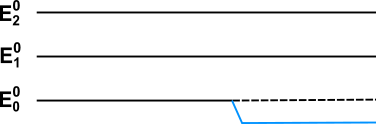
\includegraphics[width=0.37\textwidth]{energystate} % Replace with your image file
    \label{fig:example}
\end{wrapfigure}
Se un sistema di trova al livello fondamentale $E_0^0$ nell'equazione (5.22) si ha a denominatore una grandezza $(E_0^0-E_m^0) < 0$ dato che  l'energia $E_0^0$ \`e il minimo valore che il sistema pu\`o assumere. 
In generale dalle perturbazioni al secondo ordine il livello fondamentale viene sempre abbassato.

\begin{wrapfigure}{l}{0.4\textwidth} % 'r' for right, 'l' for left
    \centering
    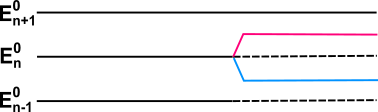
\includegraphics[width=0.37\textwidth]{energystate1} % Replace with your image file
    \label{fig:example}
\end{wrapfigure}
Per uno stato generico n-simo, si ah che per $n > m$ la perturbazione innalza il livello energetico, mentre per $m > n$ lo abbassa. Se sono presenti grandi spazi energetici tra i vari livelli si ha un contributo perturbativo minore rispetto a quelli pi\`u ravvicinati.

\subsection{Il coefficiente $C_{nn}^1$}

Per determinare il coefficiente $C^{1}_{nn}$ nella precedente sezione abbiamo scelto una normalizzazione dello stato $|\psi_n \rangle$ affinch\`e valesse la condizione (5.11). Inoltre tacitamente si \`e assunto che i termini fossero dei numeri reali, in realt\`a quando calcoliamo i coefficienti l'espressione (5.12) dovrebbe considerare il fatto che gli addendi $C_{nn}^{1}$ possono essere numeri complessi
\begin{align}
	1 & = \langle \psi_n| \psi_n \rangle = (\langle \phi_n| + \lambda \langle \psi_n|^1 +...)(|\phi_n \rangle + \lambda |\psi_n \rangle^1 +...) = \notag \\& = 1 +\lambda \langle \psi_n|^1\phi_n \rangle + \lambda \langle \phi_n|\psi_n \rangle^1 +... )=1 + \lambda(C^{1*}_{nn} + C_{nn}^1)+...
\end{align} 
 di conseguenza
 \begin{equation}
  C_{nn}^{1*} + C_{nn}^1 = 0
 \end{equation}
che equivale al sistema di equazioni

\begin{equation}
	\left \{ \begin{array}{l}
		Re(C_{nn}^1) = 0 \\[0.3cm]
		C_{nn}^1 = i\theta \quad \theta \in \mathbb{R}
	\end{array} \right.
\end{equation}
Dunque riscrivendo l'espansione dello stato $|\psi_n \rangle$ rispetto ai risultati in (5.17) abbiamo che
\begin{align*}
	|\psi_n \rangle & = | \phi_n \rangle  + \lambda (C_{nn}^1 | \psi_n \rangle + \sum_{m \neq n}C_{nm}^1 |\phi_m \rangle +...)+... = \\[0.5cm]
	& =(1+ \lambda C_{nn}^1)|\phi_n \rangle + \lambda\sum_{m \neq n}C_{nm}^1 |\phi_m \rangle +...)+... =   
\end{align*}
il termine $1+ \lambda C_{nn}^1 = 1 + \lambda i \theta$ coincide con lo sviluppo di Taylor arrestato al primo ordine della funzione $e^{i\lambda \theta}$ e quindi l'espressione precedente diventa
\begin{equation*}
	= e^{i \lambda \theta} (|\phi_n \rangle  + \lambda \sum_{m \neq n}C_{nm}^1|\psi_m \rangle +.. ) + ...
\end{equation*}
quindi abbiamo dimostrato che $C_{nn}^1$ non \`e necessariamente un termine nullo, ma pu\`o coincidere con un numero complesso di modulo unitario, che introduce un termine di fase che in meccanica quantistica pu\`o essere considerato trascurabile.

\section{Teoria delle perturbazioni indipendenti dal tempo degeneri}

Il problema \`e il medesimo di quello trattato nella sezione precedente solo che in questo caso assumiamo che i livelli energetici ammettano degenerazione.
Da un punto di vista qualitativo se $E_n^0$ \`e un autovalore degenere ci aspettiamo che i livelli reali siano sovrapposti e che l'introduzione di una perturbazione li separi.

Assumiamo che lo stato $E_n^0$ associato al sistema imperturbato possieda una degenerazione di  grado $g$; questo vuol dire che esiste un insieme di dimensione $g$ di autostati associati allo stesso autovalore.
\begin{equation}
	 \{ |\phi_n \rangle, |\phi_{n^1} \rangle, ....,|\phi_{n^g} \rangle \} 
\end{equation}
tutti associati al medesimo autovalore $E^0_{D}$,
\begin{equation*}
	E_n^0 = E_{n^1}^0 = \ldots =E_{n^g}^0 \equiv E_{D}^0
\end{equation*}
In questo caso a priori non possiamo imporre la condizione che 
\begin{equation}
	\lim_{\lambda \to 0 } |\psi_n \rangle = |\phi_n \rangle 
\end{equation}
siccome non sappiamo a quali valori dell'insieme (5.26) la funzione di stato $|\psi_n \rangle $ va a coincidere al ridursi del coefficiente perturbativo. Potrebbe anche convergere ad una loro combinazione lineare 
\begin{equation}
|\varphi\rangle=\left\langle\phi_n \mid \varphi\right\rangle\left|\phi_n\right\rangle+\left\langle\phi_{n^{\prime}} \mid \varphi\right\rangle\left|\phi_{n^{\prime}}\right\rangle+\ldots+\left\langle\phi_{n^{\prime \prime \ldots \prime \prime}}\mid \varphi\right\rangle\left|\phi_{n^{\prime \prime\ldots \prime \prime}}\right\rangle
\end{equation}
al tendere $\lambda \to 0 $. 
Data questa ambiguit\`a possiamo anche definire l'equazione del sistema senza indici
\begin{equation*}
	\hat{H}(\lambda)|\psi(\lambda) \rangle = E(\lambda)|\psi(\lambda) \rangle
\end{equation*}
ed espandiamo lo stato $|\psi \rangle $ rispetto alla base $\{|\phi_k \rangle \}$ isolando esplicitamente i contributi dati dagli stati degeneri associati al medesimo autovalore $E_{D}^0$
\begin{equation}
	|\psi(\lambda) \rangle = \sum_{m \in D} C_{m}(\lambda)|\phi_m \rangle + \sum_{k \not \in D}C_k(\lambda)|\phi_k \rangle
\end{equation}
dove $D = \{1,\ldots,g \}$ fa riferimento agli indici che identificano gli autostati degeneri.
Imponiamo la condizione per cui 
\begin{equation}
\lim_{\lambda \to 0} \equiv |\psi^0 \rangle = |\varphi \rangle 	
\end{equation}
dove, per definizione
\begin{equation}
	|\varphi \rangle = \sum_{m \in D} \langle \phi_m | \varphi \rangle |\phi_m \rangle  \quad \text{e} \quad \langle \varphi \mid \varphi \rangle = 1
\end{equation}
Dell'espressione (5.31) esistono almeno $g$ combinazioni lineari indipendenti possibili. Posto $\lambda = 0$ e utilizzando il risultato (5.30) abbiamo che l'equazione (5.29) assume la forma 
\begin{align}
	|\psi^0 \rangle & = \sum_{m \in D}C_{m}^0|\phi_m \rangle + \sum_{k \not \in D}C_{k}^0|\phi_k \rangle = \notag \\[0.5cm]
	& =  \sum_{m \in D} \langle \phi_m | \varphi \rangle |\phi_{m} \rangle 
\end{align}
dove abbiamo definito $C_{m}^0 \equiv C_m(\lambda = 0)$. Tale risultato ci dice che 
\begin{equation*}
	C_{k}^0 = \left \{ \begin{array}{l}
		\langle \phi_k|\varphi \rangle \quad k \in D \\[0.3cm]
		0 \quad \quad \quad \; k \not \in D
	\end{array}\right.
\end{equation*}
Ora procediamo come nel caso non degenere. Innanzitutto abbiamo che 
\begin{equation}
	(E - E_k^0) C_k = \lambda \sum_{m} V_{km}C_{m}
\end{equation}
Espandendo in serie di potenze coefficienti ed energie abbiamo 
\begin{equation*}
	C_k(\lambda) = C_k^0 + \lambda C_{k}^2 + \lambda^2 C_{k}^2 + \ldots 
\end{equation*}
 e
 \begin{equation*}
 	E(\lambda) = E_{D}^0 + \lambda E^1 + \lambda^2 E^2 + \ldots 
 \end{equation*}
 Sostituendo le due equazioni in (5.33) e raccogliendo i termini associati alla stessa potenza, abbiamo che 
 \begin{align}
0 & =  C_k^0\left(E_D^0-E_k^0\right) \notag \\[0.5cm]
& +\lambda\left[C_k^0 E^1+C_k^1\left(E_D^0-E_k^0\right)-\sum_m V_{k m} C_m^0\right] \notag \\[0.5cm]
& +\lambda^2\left[C_k^0 E^2+C_k^2\left(E_D^0-E_k^0\right)+C_k^1 E^1-\sum_m V_{k m} C_m^1\right]+\ldots
\end{align}
I coefficienti per ogni potenza di $\lambda$ devono essere nulli. 

\subsection{Correzioni al primo ordine $\mathcal{O}(\lambda)$}
Al primo ordine abbiamo che i coefficienti sono nulli quando valgono le seguenti condizioni 
\begin{align}
	& \sum_{m \in D} V_{km} \langle \phi_m|\varphi \rangle = E^1 \langle \phi_k| \varphi \rangle \quad \quad \;\; k \in D \\[0.5cm]
	& C_k^1(E_D^0-E_k^0) = \sum_{m \in D} V_{km} \langle \phi_{m} | \varphi \rangle \quad  k \not \in D
\end{align}
Chiaramente, le grandezze $V_{km}$ con $k,m \in D$, possono essere interpretate come elementi di una matrice $g \times g$. La relazione (5.35) pu\`o essere vista come un equazione rispetto agli autovalori che determina i $g$ autovalori $\{ E_{a}^2 \} = \{ E_{1}^1,E_{2}^2,...,E_{g}^1\} $ e i corrispondenti $g$ autostati $\{|\varphi_a \rangle  \} = \{ |\varphi_1 \rangle, |\varphi_2 \rangle ,...,|\varphi_g \rangle \} $. L'equazione (5.35) implica che in presenza di una perturbazione del sistema, l'insieme dei $g$ autostati degeneri $|\phi_n \rangle , |\phi_{n'} \rangle, \ldots , |\phi_{n^{'' \ldots ''}} \rangle  $ con autovalori $E_{D}^0$, vengono trasformati rispetto al primo ordine in un nuovo insieme di autostati $|\varphi_{1} \rangle, \ldots | \varphi_{g} \rangle $ con autovalori $E_{D}^0 + \lambda E_{1}^1,E_{D}^0 + \lambda E_{2}^1, \ldots,E_{D}^0 + \lambda E_{g}^1$.
Assumendo che i nuovi autovalori sia non degeneri, possiamo dire che \textit{la perturbazione ha rimosso la degenerazione}.

\section{Effetto Stark - Atomo d'idrogeno in un campo elettrico costante}

In questa sezione studiamo l'effetto Stark nell'idrogeno come esempio di teoria delle perturbazioni per uno stato legato. L'effetto Stark riguarda il comportamento degli atomi in presenza di un campo elettrico costante. 

Le prime osservazioni della divisione delle linee spettrali di un atomo per via dell'interazione con un campo elettrico sono state fatte da Stark nel 1913, che gli valse il premio Nobel nel 1919.
\newpage

\subsection{Sistema imperturbato}

Abbiamo un sistema costituito da un nucleo attorno al quale orbita un solo elettrone, ignorando lo spin delle particele, vogliamo studiare lo stato fondamentale dell'atomo d'idrogeno.

L'atomo a singolo elettrone viene modellato usando la Hamiltoniana che esprime un sistema a forza centrale 
\begin{equation}
	\hat{H}_0 = \frac{p^2}{2m} + V_0(r)
\end{equation}
dove per l'idrogeno abbiamo che
\begin{equation*}
	V_0 (r) = - \frac{e^2}{r}
\end{equation*}
Prima di iniziare a descrivere il sistema perturbato, abbiamo bisogno di capire il comportamento di quello imperturbato, a partire dalle sue energie, autostati e degenerazioni. Nel modello elettrostatico, i livelli di energia del sistema imperturbato sono descritti dalla formula Bohr
\begin{equation*}
	E_n = - \frac{1}{2n^2}\frac{e^2}{a_0} = -\frac{E_0}{n^2} \quad n \in \mathbb{N}
\end{equation*}
dove il termine $a_0$ indica il raggio di Bohr ed $E_0 = 13,6 \; eV$ l'energia associata allo stato fondamentale. Per l'atomo d'idrogeno gli atuovalori hanno una degenerazione di $n^2$. Gli autostati associati sono dati da 
\begin{equation*}
	|nlm \rangle = \psi_{nlm}(\bold{x}) = R_{nl}Y_{lm}(\theta,\phi)
\end{equation*}
dove le funzioni $Y_{lm}(\theta, \phi)$ sono armoniche sferiche.

\subsection{Potenziale}
Scriviamo la forza esterna $\bold{F}$ dovuta al campo elettrico esterno ed assumiamo che abbia orientazione lungo l'asse $\hat{u}_{z}$,
\begin{equation*}
	\bold{F} = F \hat{u}_{z}
\end{equation*}
Di conseguenza il potenziale della perturbazione ha forma
\begin{equation*}
	V_1 = q \phi = - q\bold{F} \cdot \bold{x} = eFz
\end{equation*}
dove si \`e considerato $q = -e $. Il potenziale imperturbato $V_0$ dipende da $r$, mentre quello perturbato $V_1$ dipende da $z$, di conseguenza abbiamo che la perturbazione del sistema rompe la simmetria di rotazione $SO(3)$ presente nel sistema imperturbato.

\subsection{Effetto Stark nello stato fondamentale}

Iniziamo la trattazione del caso perturbativo partendo dallo stato fondamentale dell'atomo di idrogeno; in notazione chimica coincide con la configurazione $1s$ che corrisponde all'autostato $| 100\rangle $. Siccome allo stato fondamentale non \`e presente degenerazione la correzione di energia al prima ordine \`e data da 
\begin{equation*}
	E^1_{0} = \langle 100|V |100 \rangle = 0 
\end{equation*}
che risulta essere nulla poich\`e 
\begin{equation*}
	\langle 100| eEz | 100 \rangle = eE \langle 100|z|100 \rangle  = eE\frac{1}{4 \pi} \int_{-\infty}^{\infty}dz z = 0 
\end{equation*}
dato che $z$ \`e una funzione dispari. Quindi possiamo concludere che al primo ordine per lo stato fondamentale dell'idrogeno non \`e presente una perturbazione al primo ordine dell'energia e di conseguenza nessun effetto Stark.

\subsection{Effetto Stark negli stati eccitati dell'idrogeno}

Gli stati eccitati dell'idrogeno per $n \geq 2$ hanno una degenerazione tra gli stati con opposta parti\`a, dato che $l = 0,...,n-1$ e la parti\`a \`e pari per $l$ parti e dispari per $l$ dispari.  In accordo con la teoria descritta in precedenza per le perturbazioni di secondo ordine, la variazione dei livelli di energia $E_n$ \`e data dagli autovalori della matrice $n^2 \times n^2$, indicizzata da $(lm)$ e $(l'm')$
\begin{equation*}
	\langle nlm| eFz|nl'm' \rangle 
\end{equation*}





